\documentclass{article}

\usepackage{listings}
\usepackage[utf8]{inputenc}
\usepackage[spanish]{babel} % Agregar es-nodecimaldot si hay problemas con el separador de decimales y de miles
% \usepackage{noto-mono} % Tipografía "Noto Sans Mono" para monospace
\usepackage{amsmath, amsbsy, amssymb} % Agregar cuando se necesiten: amscd, amssymb, amsthm, latexsym
\usepackage{enumerate}
\usepackage{graphicx}
\usepackage{multicol}
\usepackage{svg}
\usepackage{tabularx}
\usepackage{algorithm}
\usepackage{algpseudocode}
\usepackage{caption}
\usepackage{etoolbox}

% Tamaño de hoja y márgenes
\usepackage[a4paper,top=1cm,bottom=2cm,left=1cm,right=1cm]{geometry}
\setlength{\parindent}{0em}
\setlength{\parskip}{1em}
\setlength{\intextsep}{1em}
\setlength{\abovedisplayskip}{1em}
\setlength{\belowdisplayskip}{1em}
\setlength{\abovedisplayshortskip}{1em}
\setlength{\belowdisplayshortskip}{1em}

% Numeración de las secciones y el índice
\setcounter{tocdepth}{1}
\renewcommand{\thesubsection}{\thesection.\alph{subsection}}

% Color de los links externos
\usepackage{hyperref}
\hypersetup{colorlinks=true, linkcolor=black, urlcolor=blue}

% Permite math mode adentro de listings (bloques de "código")
\usepackage{listings}
\lstset{
    inputencoding=utf8,
    extendedchars=\true,
    basicstyle=\ttfamily\small,
    mathescape,
    literate=%
        {á}{{\'a}}1
        {é}{{\'e}}1
        {í}{{\'i}}1
        {ó}{{\'o}}1
        {ú}{{\'u}}1
        {Á}{{\'A}}1
        {É}{{\'E}}1
        {Í}{{\'I}}1
        {Ó}{{\'O}}1
        {Ú}{{\'U}}1
        {ñ}{{\~n}}1
        {Ñ}{{\~N}}1
}

% Alias para íconos/símbolos
\usepackage{pifont}
\newcommand{\xmark}{\color{purple}\ding{54}}

% Otros alias
\newcommand{\xor}{\oplus}
\newcommand{\nor}{\downarrow}
\newcommand{\opsub}[2]{\ensuremath{#1_{\mathrm{#2}}}}
\newcommand{\yLuego}{\opsub{\land}{\scriptscriptstyle{L}}}
\newcommand{\oLuego}{\opsub{\lor}{\scriptscriptstyle{L}}}
\newcommand{\implicaLuego}{\opsub{\implies}{\scriptscriptstyle{L}}}
\renewcommand{\implies}{\Rightarrow}

% Columna "x" tiene fondo amarillo
\usepackage{colortbl}
\newcolumntype{x}{>{\columncolor[HTML]{FFF2CC}}c}

% Tipografía para los algoritmos
\AtBeginEnvironment{algorithmic}{\small}

% Saca sufijo "Algorithm X"
\captionsetup[algorithm]{labelformat=empty}

% Alias para algoritmos
\newcommand{\Complexity}[1]{\textbf{Complejidad}: #1}
\newcommand{\Pre}[1]{\textbf{Pre} $\equiv$ \{#1\}}

\setlength{\parindent}{0pt}

\title{Práctica 1}
\author{Representación de la información}
\date{Agosto 2022}

\begin{document}

\maketitle

\section*{Ejercicio 1}

\subsection*{a)}
\begin{table}[htbp]
    \begin{tabular}{|c|c|c|}
    \hline
    \textbf{p} & \textbf{q} & \textbf{$((pq) + (p\overline{q}))$} \\ \hline
    F          & F          & \textbf{F}                    \\ \hline
    F          & T          & \textbf{F}                    \\ \hline
    T          & F          & \textbf{T}                    \\ \hline
    T          & T          & \textbf{T}                    \\ \hline
    \end{tabular}
\end{table}

\subsection*{b)}

\begin{table}[htbp]
    \begin{tabular}{|c|c|c|c|l|}
    \hline
    \textbf{x} & \textbf{y} & \textbf{z} & \textbf{((x + y) . ((x + ¬y) . (¬x + z)))} & xz \\ \hline
    F          & F          & F          & F                                          & F  \\ \hline
    F          & F          & T          & F                                          & F  \\ \hline
    F          & T          & F          & F                                          & F  \\ \hline
    F          & T          & T          & F                                          & F  \\ \hline
    T          & F          & F          & F                                          & F  \\ \hline
    T          & F          & T          & T                                          & T  \\ \hline
    T          & T          & F          & F                                          & F  \\ \hline
    T          & T          & T          & T                                          & T  \\ \hline
    \end{tabular}
    \end{table}

Tablas de verdad generator: \url{https://web.stanford.edu/class/cs103/tools/truth-table-tool/}
\section*{Ejercicio 2}

\begin{align*}
    x \oplus (y.z) &= (x \oplus y).(x \oplus z) \\
    x \oplus (y.z) &= ((\overline{x}.y) + (x.\overline{y})).((\overline{x}.z) + (x.\overline{z})) \\
    x \oplus (y.z) &= (\overline{x}.y.z) + (y.\overline{z}) + (\overline{y}.z) + (x.\overline{y.z}) \\
    x \oplus (y.z) &= (\overline{x}.y.z) + (x.\overline{y.z}) \\
    x \oplus (y.z) &= x \oplus (y.z)
\end{align*}

\section*{Ejercicio 3}

Dada una base $b$, y siendo $r_1$ y $r_2$ dos digitos a sumar tales que $ 0 \leq r_1, r_2 \leq b $ habrá un acarreo mayor a 1 si:

\begin{align*}
    r_1 + r_2 + 1 &\geq 2b \\
\end{align*}

Pero $ r_1 < b $ y $ r_2 < b $ luego, $ r_1 + r_2 + 1 < 2b $ y por lo tanto no puede haber acarreo distinto de 0 o 1.
\section*{Ejercicio 5}

\begin{itemize}
    \item $ 0_{10} = 00000000_{sm} = 00000000_{c2} $
    \item $ -1_{10} = 10000001_{sm} = 11111111_{c2} $
    \item $ -1_{10} = 1000000000000001_{sm} = 1111111111111111_{c2} $
    \item $ 255_{10} = 11111111_{ss} = 000000011111111_{c2} $
    \item $ -128_{10} = 10000000_{c2} = 1111111110000000_{c2} $
    \item $ 128_{10} = 10000000_{ss} = 0000000010000000_{c2} $
\end{itemize}
\section*{Ejercicio 6}

\begin{itemize}
    \item $ r = -65_{c2} = -63_{sm} $
    \item $ s = -128_{c2} = -0_{sm} $
    \item $ s = -1_{c2} = -127_{sm} $
\end{itemize}
\section*{Ejercicio 7}

\begin{itemize}
    \item $ 2 = 0010 $
    \item $ -5 = 1101 $
    \item $ 0 = 0000 $
\end{itemize}

\subsection*{a)}

Invertidos

\begin{itemize}
    \item $ 2 = 1101 = -5 $
    \item $ -5 = 0010 = 2 $
    \item $ 0 = 1111 = -1 $
\end{itemize}
\section*{Ejercicio 8}

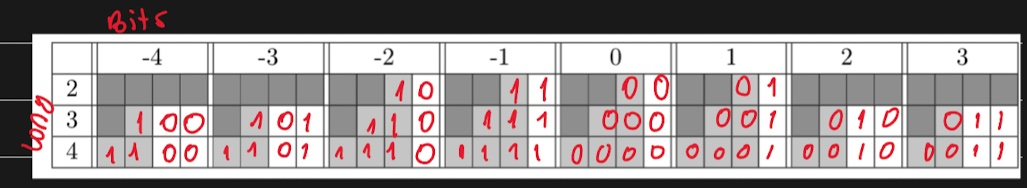
\includegraphics[width=18cm]{./static/P1E8.jpg}

En los positivos las posiciones que "sobran" son iguales a 0 mientras que en os negativos son iguales a 1.
\section*{Ejercicio 9}

\begin{itemize}
    \item $ 0000 + 0001 $
    \item $ 0011 + 0001 $
    \item $ 1111 + 0001 $
    \item $ 1000 + 1000 $
    \item $ 0001 + 1111 $
    \item $ 0000 + 0000 $
\end{itemize}

\section*{Ejercicio 10}

El número 1000 en complemento a 2 se representa -8 pero en signo magnitud $ -8 = 11000 $ luego no puede ser representado por una cadena de 4 digitos.

No ocurre al reves.
\section*{Ejercicio 11}

El sistema de signo + magnitud es un sistema de representación biyectivo donde la cantidad de negativos y positivos es la misma para un número dado de bits.

\end{document}